\chapter{Methods}
\label{c:methods}

This chapter provides with an overview of the methodological framework (the combination of methods) used to achieve the stated \nameref{s:intro:aim-objectives} in each of the following sections. \sref{s:methods:vision} deals with the sustainable mobility vision development. The requirements (changes) for the transition were derived using the method described in \sref{s:methods:backcasting}. \sref{s:methods:clds} explains the methodology that was used to identify the policy resistance mechanisms in the current system and, finally, \sref{s:methods:mlp-policies} explains the analytical framework used to design the policy recommendations for the transition. A graphical overview of the methodological framework is given in \fref{f:thesis-aim-methods}.
%TODO delete the follwing: \parencite{hoejer2000_Determinismbackcastingfuture,dreborg1996_Essencebackcasting,dortmans2005_Forecastingbackcastingmigration,kok2011_Combiningparticipativebackcasting}

\section[Qualitative narratives]{Qualitative narratives: setting the vision}
\label{s:methods:vision}
Concerning the first of the objectives described in the Introduction chapter, no formal method is used to \emph{obtain} the ``vision'' of a future mobility system. The vision is not derived from any kind of forecasting or modelling tool. Instead, a literature review was performed at the beginning of the thesis, searching for papers with the keywords ``sustainable'', ``mobility'' and ``paradigm''. While several articles were found (e.g., \textcite{banister2008_sustainablemobilityparadigm}), little or none of them actually gave a clear picture of a \emph{future paradigm} of sustainable mobility. Most of the papers consisted only on discussions regarding some of the aspects that could conform a sustainable mobility paradigm. Therefore, the decision was taken to build a new vision on already existing research. The final choice for the basis of the vision is the long-term scenario framework by the \gls{IPCC} (see \sref{s:results:ssp1-mob} for more detail). This framework consists on five different qualitative narratives that are then translated into sets of (quantitative) assumptions in the global climate change assessment models (\gls{IAM}).

\begin{figure}
\centering
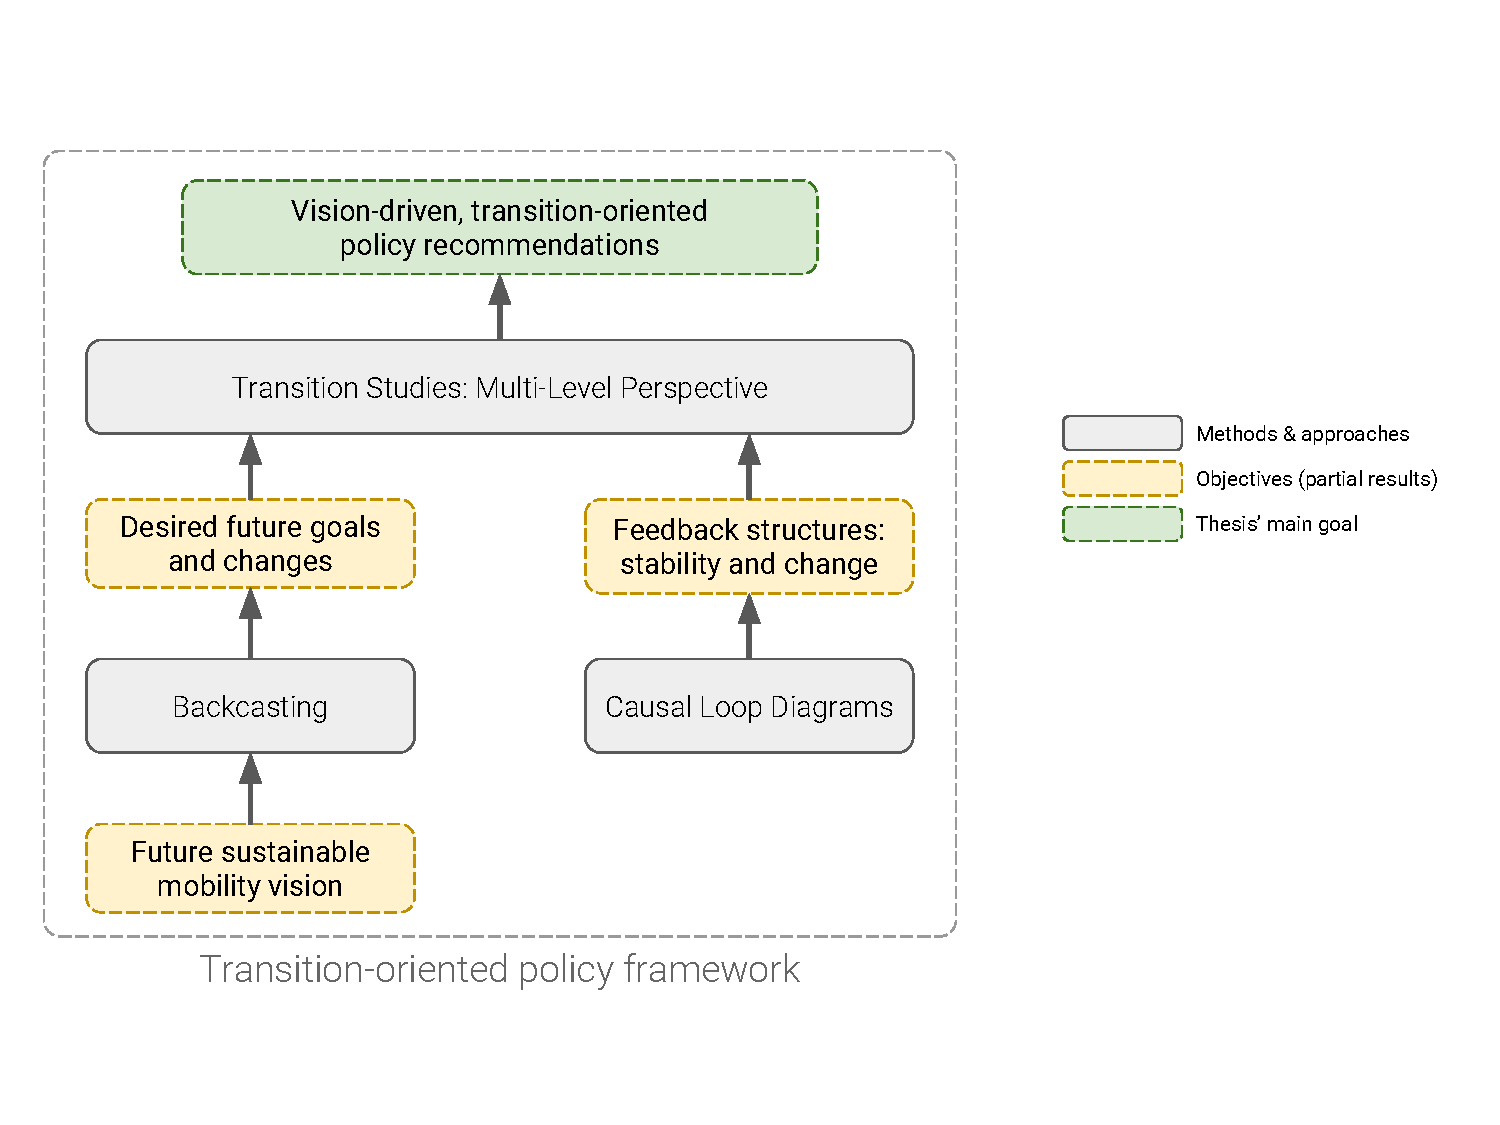
\includegraphics[width=0.8\linewidth,trim=0 2cm 0 2cm,clip]{figures/methods-goals.pdf}
\caption[Methodological framework]{Methodological framework, linking methods to objectives and showing the flow of information until the final aim (policy recommendations) is reached.}
\label{f:thesis-aim-methods}
\end{figure}

The vision in this thesis is developed following the same method as \textcite{oneill2017_roadsaheadNarratives} did for the IPCC scenarios: through a \emph{qualitative narrative} in which the aspects of the sustainable mobility paradigm are explained qualitatively. With respect to how the vision is developed, it is done so by building upon the foundations of the SSP1 scenario by the IPCC, in combination with insights gained from the literature. However, the structural elements of the narrative are withdrawn from the IPCC's storyline.

The fact that the IPCC scenarios are developed from a set of narratives actually makes them easier to transform into a ``vision'' than more traditional scenarios: the IPCC scenarios explore final \emph{states}, rather providing with forecasts. Drawing on the scenario typology built by \textcite{boerjeson2006_Scenariotypestechniques}, IPCC's would fall under the ``exploratory'' scenarios category, while the actual approach of the backcasting process (see \sref{s:methods:backcasting}) in this thesis would fall under the ``normative'' category. Despite these seem not to fit, the truth is that in order to build the vision for the backcasting in \ssref{ss:results:ssp1-mob-development}, it is very useful to start from the ground of an already developed, consistent and acknowledged exploration of a \emph{possible} future. This way, a lot of assumptions are already justified and the whole vision frame is not purely speculative in nature.

\section[Backcasting]{Backcasting: analysing the transition pathway}
\label{s:methods:backcasting}
In order to obtain the desired pathway of the transition to the vision (Obj. 2), the \emph{backcasting} method was used. Backcasting processes are the inverse of traditional forecasts. Instead of extrapolating current trends into the future, they start from a defined end-state or goal that represents a desirable and somehow plausible future. Then, either through stakeholder participatory workshops, expert panels or ``in-house'' development processes, a set of intermediate goals are set at whatever time-frames are required. The backcasting process is finalised when the identification of the trends and changes that separate the desired future and the current state of the system under study \parencite{dreborg1996_Essencebackcasting}. Backcasting usually serves a normative purpose and, most importantly, they are usually rhetorical instead of analytical. The strength of this methodology lies in the ability to extend the range of possibilities under consideration \parencite{mcdowall2006_Forecastsscenariosvisions}.

The main reason behind this choice was the fact that backcasting is, in itself, a normative methodology for futures analysis \parencite{boerjeson2006_Scenariotypestechniques,mcdowall2006_Forecastsscenariosvisions}, something required for filling the gaps identified by this thesis (and to help in the derivation of the policy recommendations for Obj. 4). Additionally, backcasting is also a more promising method when great changes are expected or required, which is the case of a transition to sustainable mobility \parencite{hoejer2000_Determinismbackcastingfuture}. Note that, due to resource limitations and time budgets, the backcasting process was not performed in a participatory manner. No stakeholders were involved, nor an expert panel, thus becoming a limitation in the power of the study, as discussed in \cref{c:discussion}.

\begin{figure}
\centering
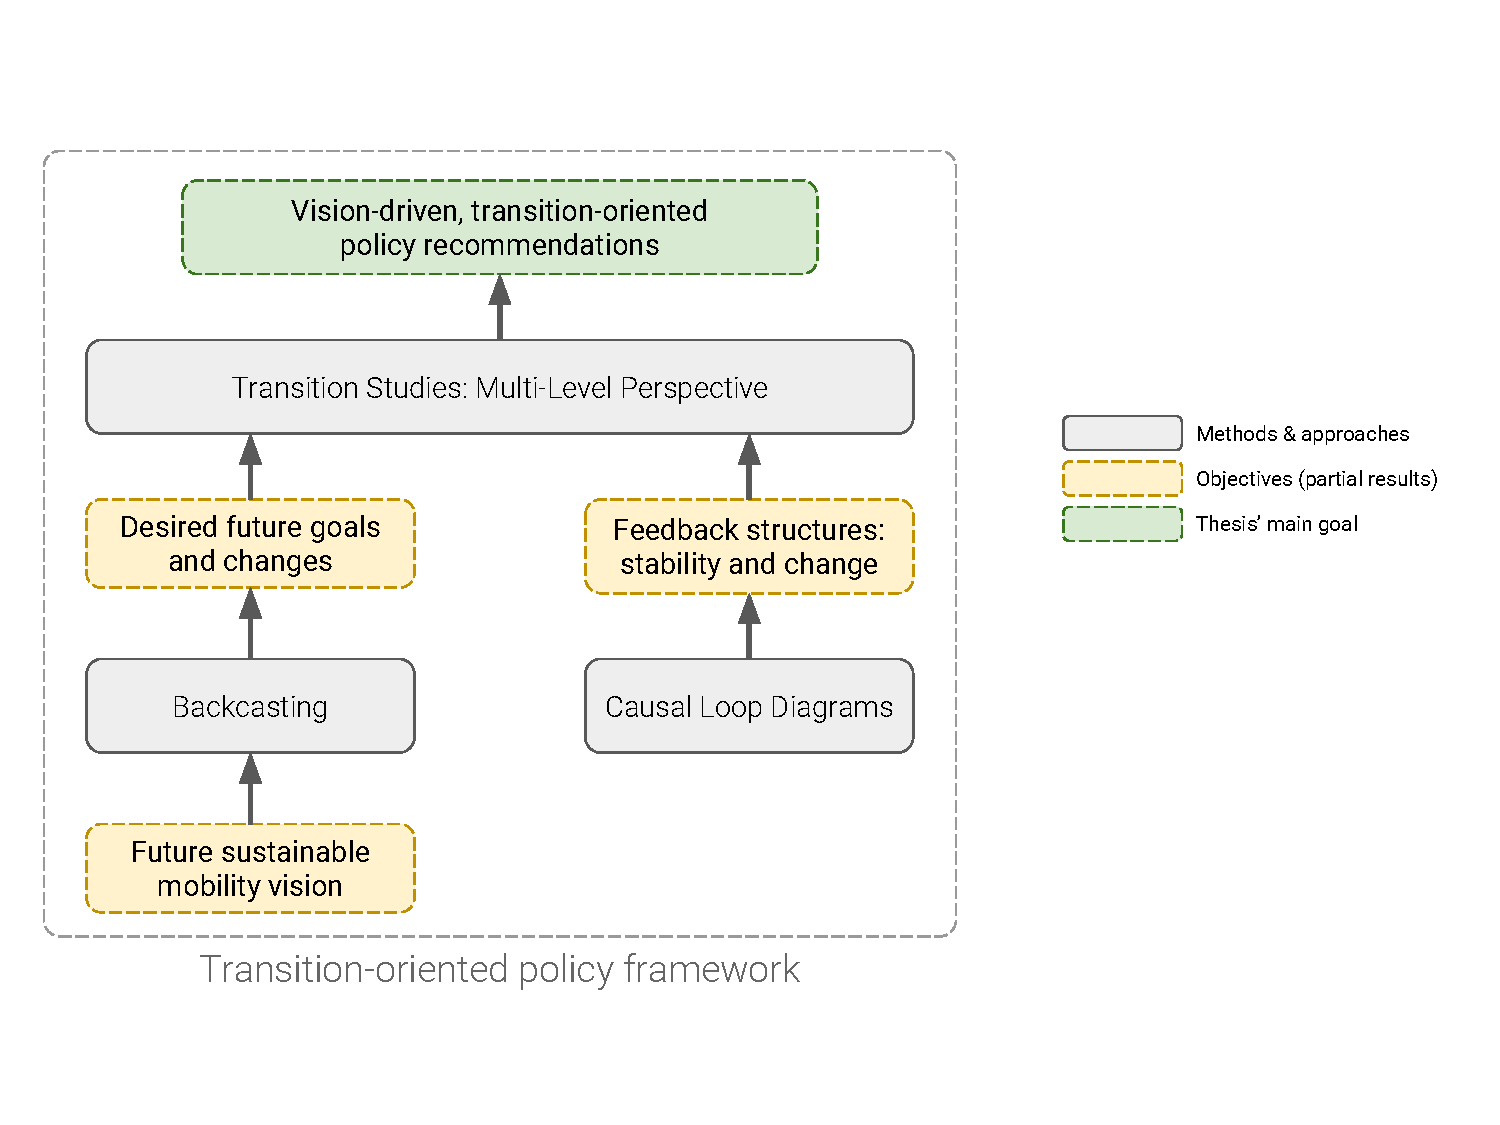
\includegraphics[width=0.7\linewidth,trim=0 1cm 0 1cm,clip]{figures/methods-goals.pdf}
\caption[Methodological framework]{Methodological framework, linking methods to objectives and showing the flow of information until the final aim (policy recommendations) is reached.}
\label{f:thesis-aim-methods}
\end{figure}

\section[Causal Loop Diagrams]{Causal Loop Diagrams: analysing current policy resistance}
\label{s:methods:clds}
The third objective of the thesis is the analysis of policy resistance mechanisms of the current mobility system (Obj.~3). The chosen method to do this is the development of \emph{\glspl{CLD}}. CLDs are the first of the steps used in the broader methodological framework of System Dynamics \parencite{ghosh2015_DynamicSystemsEveryone}. Due to the difficulty of dealing with entire systems, their internal dynamics and the emergent systemic behaviour patterns, such as feedback loops, rebound effects and hidden causalities, simple linear/mechanistic (conceptual) models are simply insufficient to provide a complete system picture \parencite{forrester1972_CounterintuitiveBehaviorSocial}. In this regard, the field of System Dynamics can help capture such structures and cause-effect chains \parencite{hjorth2006_Navigatingtowardssustainable}. An interesting and relevant example of what System Dynamics modelling can achieve is the World3 model in \emph{The Limits to Growth} report from the Club of Rome \parencite{meadows1972_LimitsGrowthReport}, where the global food, industrial, population, non-renewable resources and pollution systems were assessed with regards to the limits of the Earth's ecosystems.

%\todowarning{Provide a simple example of a CLD here}

CLDs consist of variables linked by causal relations, which can either be positive (directly proportional) or negative (inversely proportional). Note that these causal links are not quantified in a CLD: the quantification step (attaching equations to the relations) is performed in a further modelling stage, giving rise to ``stock-flow'' models \parencite{sterman2000_BusinessDynamics}. An important concept is necessary to interpret the diagrams in the \nameref{c:results} chapter: feedback \emph{loops}. These structures are cycles of causes and effects (variables) that are behind the dynamic behaviour of systems. These feedback mechanisms can either \emph{reinforce} or \emph{balance} the overall behaviour of the system. Reinforcing loops are responsible for the exponential growth (or shrinkage) of the involved variables, whereas balancing loops orient the variables asymptotically towards a ``target'' level \parencite{sterman2000_BusinessDynamics}.

%\todowarning{Provide a figure with the reinforcing and balancing system behaviours}

With regards to how the CLDs were developed in this thesis specifically, the methodology followed was very similar to the process described by \textcite{laurenti2015_TowardsAddressingUnintended}. A first step was taken to ``frame the challenge'', this is, to decide what was the problem or issue to tackle---in the case of this thesis, the goal was to identify feedback structures within the socio-cultural dimensions of mobility that reinforce and stabilise the current system. After this, a ``core'' conceptual model (the CLD) was developed on the basis of insights gained from the literature. System boundaries were expanded from the core model in order to capture enough causal links as to understand the system's feedback structure. The final step was to ``prune'' the model, shrinking the boundaries so that it became simpler and easier to convey to the reader. The analysis of the resilience mechanisms and windows of opportunity for change (Obj.~3) is embedded both in the section where the CLDs are developed (\sref{s:results:autolock-model}) and in the integration through the transitions perspective (\sref{s:results:characterizing-transition}) that gives birth to the policy recommendations (\sref{s:results:policy-recommendations}).

\section[Multi-Level Perspective]{Multi-Level Perspective: deriving transition-oriented policy recommendations}
\label{s:methods:mlp-policies}
Regarding the ultimate goal of deriving policy recommendations (Obj.~4 in \sref{s:intro:aim-objectives}), no particular welfare (economic) assessment tool was used. The recommendations are general guidelines, not specific numbers on, for example, environmental taxes, thus the decision was made to avoid using a formal economic assessment method. Instead, the policies were \emph{informed} by the transition studies perspective \parencite{kemp2007_Transitionmanagementas}, which integrates the results of the backcasting process (the transition pathway) and the analysis of the feedback structures in the current mobility system through the use of CLDs.

The integration of the rest of the results through a transitions perspective was done by analysing those same insights through a different \emph{discourse}. The formal method used for rising the CLD and backcasting outcomes to the same discursive level is the so called \emph{\gls{MLP}}. This analytical framework defines three levels that characterise a socio-technical system \parencite{geels2001_Technologicaltransitionsas}. These levels are associated with micro, meso and macro perspectives, as portrayed in \fref{f:mlp-methods} \parencite{rotmans2001_Moreevolutionthan}:
\begin{enumeratealpha}
\item The socio-technical \emph{niche} level, at the most microscopic level of the system, is the location where radical innovation occurs. Several processes occur within the niches: the articulation of expectations (visions), the construction of stakeholder networks and learning on different dimensions (organisational, policy, technological, etc.) \parencite{geels2012_MultiLevelPerspective}.
\item The socio-technical \emph{regime} level is situated at the mesoscopic level. It is the virtual space formed by all the actors within a socio-technical system, their shared practices, rules and cultures. Infrastructure supporting the socio-technical system, as well as regulation, and technology belong to the regime level too. In the case of regimes, innovation is not radical. Instead, it is incremental and rather slow, following a pattern of ``dynamic stability''. Resilience is, thus, a key characteristic of regimes \parencite{geels2012_MultiLevelPerspective}.
\item The socio-technical landscape, at the macroscopic level, is the context in which both regimes and niches are embedded. Ideologies, culture, value hierarchies, beliefs, macroeconomic trends, the media, governance systems, etc. belong to this level. The landscape shapes, through pressures and support relations, the regimes and the niches. A characteristic of this level is the slow changes it suffers: regimes come and go, even more so niches, but it can take several decades or even centuries for change in the landscape to become apparent \parencite{rotmans2001_Moreevolutionthan,kemp2007_Transitionmanagementas,geels2012_MultiLevelPerspective}.
\end{enumeratealpha}

\begin{figure}
\centering
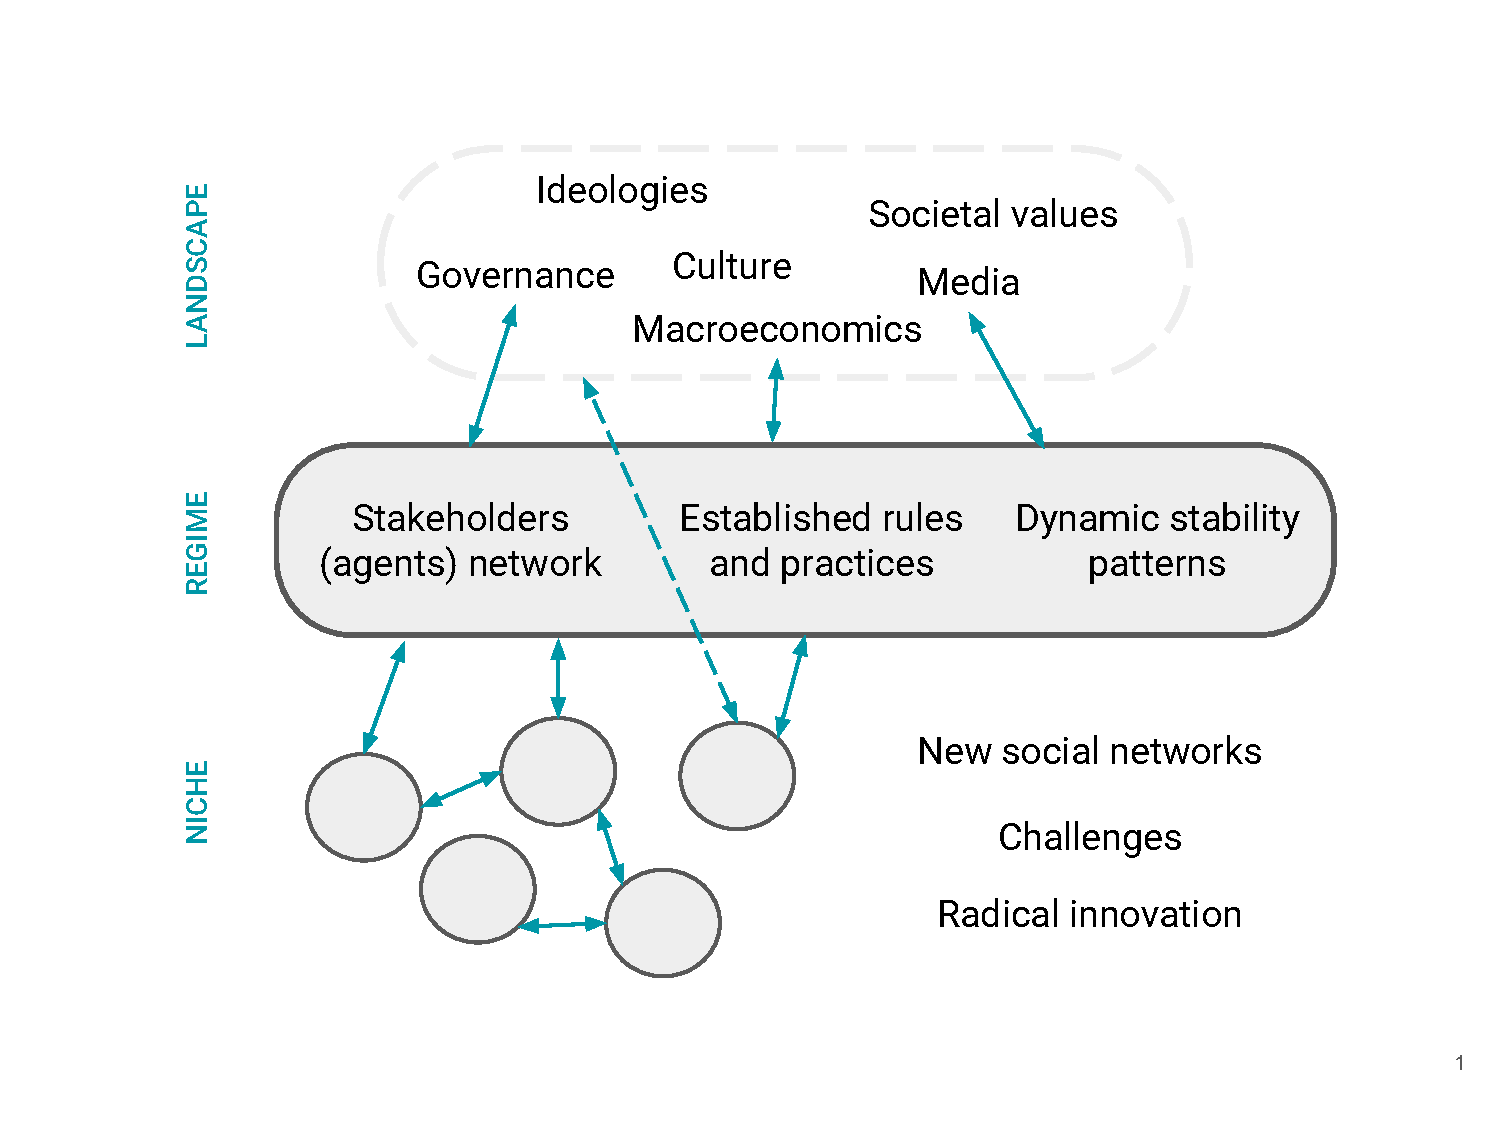
\includegraphics[width=0.8\linewidth,trim=0 2cm 0 2cm,clip]{figures/mlp.pdf}
\caption[The Multi-Level Perspective]{The Multi-Level Perspective analytical framework, with the macro, meso and micro levels visible.}
\label{f:mlp-methods}
\end{figure}

The MLP allows for a multi-dimensional analysis of mobility, because it deals with more than just technologies (or any other aspect of the system: economics, environmental impacts, regulation, etc.). This is ideal to overcome the limitations in scope of traditional transport research identified in the \nameref{s:intro:state-of-art} section. The MLP also addresses structural change by analysing how socio-technical innovations fight for dominance against established regimes. Structural change is an important element in transitions that previous mobility research (or policy) tends to obviate. The MLP also stresses the importance of the patterns of co-evolution between the landscape and regimes and niches. In particular, the MLP (and transitions studies in general) addresses the dynamics of stability and change of regimes and niches \parencite{geels2011_multilevelperspective}. This specific feature of the MLP serves very well the aim of the thesis of understanding why mobility presents policy resistance and what can be done to tackle it.

Finally, the way in which the MLP is used in the thesis is as follows: the backcasted changes (Objs.~1,2) that conform the transition pathway are described in the terms of the MLP. The feedback mechanisms that cause policy resistance in today's mobility system (Obj.~3) are then incorporated to the description and also translated into the language of the MLP. Thus, the narration of the transition path contains: (1) normative elements on a broad range of dimensions, stemming from the backcast and (2) a dynamic analysis of the forces that can hinder the transition nowadays. This MLP-inspired analysis is finally used to design a set of policy recommendations that focuses both on the long term goals and on breaking the resilience of the current mobility system that poses an obstacle to its own radical transformation (Obj.~4).